\hypertarget{chapter-1}{%
\chapter{Chapter 1}\label{chapter-1}}

This is Chapter 1. Here is one of my marvellous pictures.

\begin{figure}
\centering
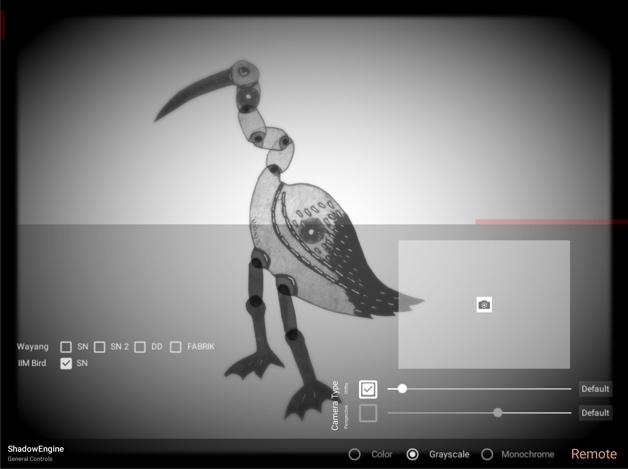
\includegraphics{assets/image053.jpg}
\caption{Horray Here's the caption.}
\end{figure}

Where is the freaking caption?

\hypertarget{sec:ch2}{%
\chapter{Chapter 2}\label{sec:ch2}}

This is Chapter 2.

\hypertarget{chapter-3}{%
\chapter{Chapter 3}\label{chapter-3}}

This is Chapter 3.

\hypertarget{tbl:table1}{}
\begin{longtable}[]{@{}lrrrr@{}}
\caption{\label{tbl:table1}Average Times for Components}\tabularnewline
\toprule
Type & Count & ø Time & Median Time & ø Commits\tabularnewline
\midrule
\endfirsthead
\toprule
Type & Count & ø Time & Median Time & ø Commits\tabularnewline
\midrule
\endhead
Atom & 9 & 1:30:23 & 0:48:00 & 13,2\tabularnewline
Molecule & 10 & 1:20:12 & 1:12:45 & 8,9\tabularnewline
Layout & 5 & 1:21:48 & 0:57:00 & 3,0\tabularnewline
Template & 5 & 2:30:30 & 2:27:00 & 4,0\tabularnewline
\bottomrule
\end{longtable}

\hypertarget{chapter-4}{%
\chapter{Chapter 4}\label{chapter-4}}

This is Chapter 4.

\autocite{kozelCloserPerformanceTechnologies2007}
